\documentclass[]{article}
\usepackage{graphicx}
\usepackage{geometry}
\geometry{
	a4paper,
	total={170 mm, 257mm},
	left=30mm,
	right=35mm,
	top=20mm,
}
%opening
\title{Physics 117 Lab 2}
\author{Shijia (Scarlett) Yu \\Lab Partner: Ryan\\Prof: Musumeci TA: Albert Brown}
\date{January 11, 2017}

\begin{document}
	\maketitle
	\paragraph { (a)} %\mbox{}\\
	We used the capacimeter to measure $C_{1}$=10.1nF =0.0101$\mu F$, and $C_{2}$ =10.4nF=0.0104$\mu F$. The capcimeter only displays in nF, but we can convert it to $\mu F$ using $1nF=10^{-9}F=10^{-3}\mu F$. \\Capacitnace in series and parallel:\\ we  connected $C_{1}$ and $C_{2}$ in series to measure $C_{s,tot}$. The calculated value for total capacitance in series is $C_{s, tot}$=$ \frac{C_{1}C_{2}}{C_{1}+C_{2}}$=$ \frac{105.04}{10.4+10.1}nF=5.12nF$. The measured total capacitance in series is 4.94nF. The calculated value for total capacitance in parallel is $C_{s, tot}$=$ C_{1}+C_{2}=20.5nF$. The measured total capacitance in parallel is 20.3nF. \\
	Reading the ceremic capcacitor: \\
	The capacitors we used have label "154 (K1C)" written on them. The last digit "4" is a multiplier, which means $10^{4}$. so "154" means $15\times10^{4}pF$. The "K1C" is just the tolerance.
	\paragraph{ (b)} 	
	We built the RC circuit with a 9.9k resistor and 0.01$\mu$F capcitor. We then drove the circuit with a 500 Hz square wave and connected the scope around the capcitor to get the output signal. The scope was put on DC coupling because otherwise the 500 Hz low frequency would be cut off by the AC coupling.\\
	 The calculated RC time constant for this circuit is $\tau =RC=(9.9\times10^{3}\Omega)(0.01\times10^{-6}F)=100\mu s$.\\ To measure the rise time of the circuit, which is the time required to go from 0\% to 63\% of its maximum voltage, we found the voltage at 63\% max and used cursors to find the $\Delta t$ between 0\% and  63\% voltage point (see Fig.1). The maximum voltage was 100mV, so we looked at the time at around 63mV.  The cursors gave us $\Delta t=108 \mu s$, which is close to the calcualted 100$\mu$ s.\\
	 	\begin{center}
	 		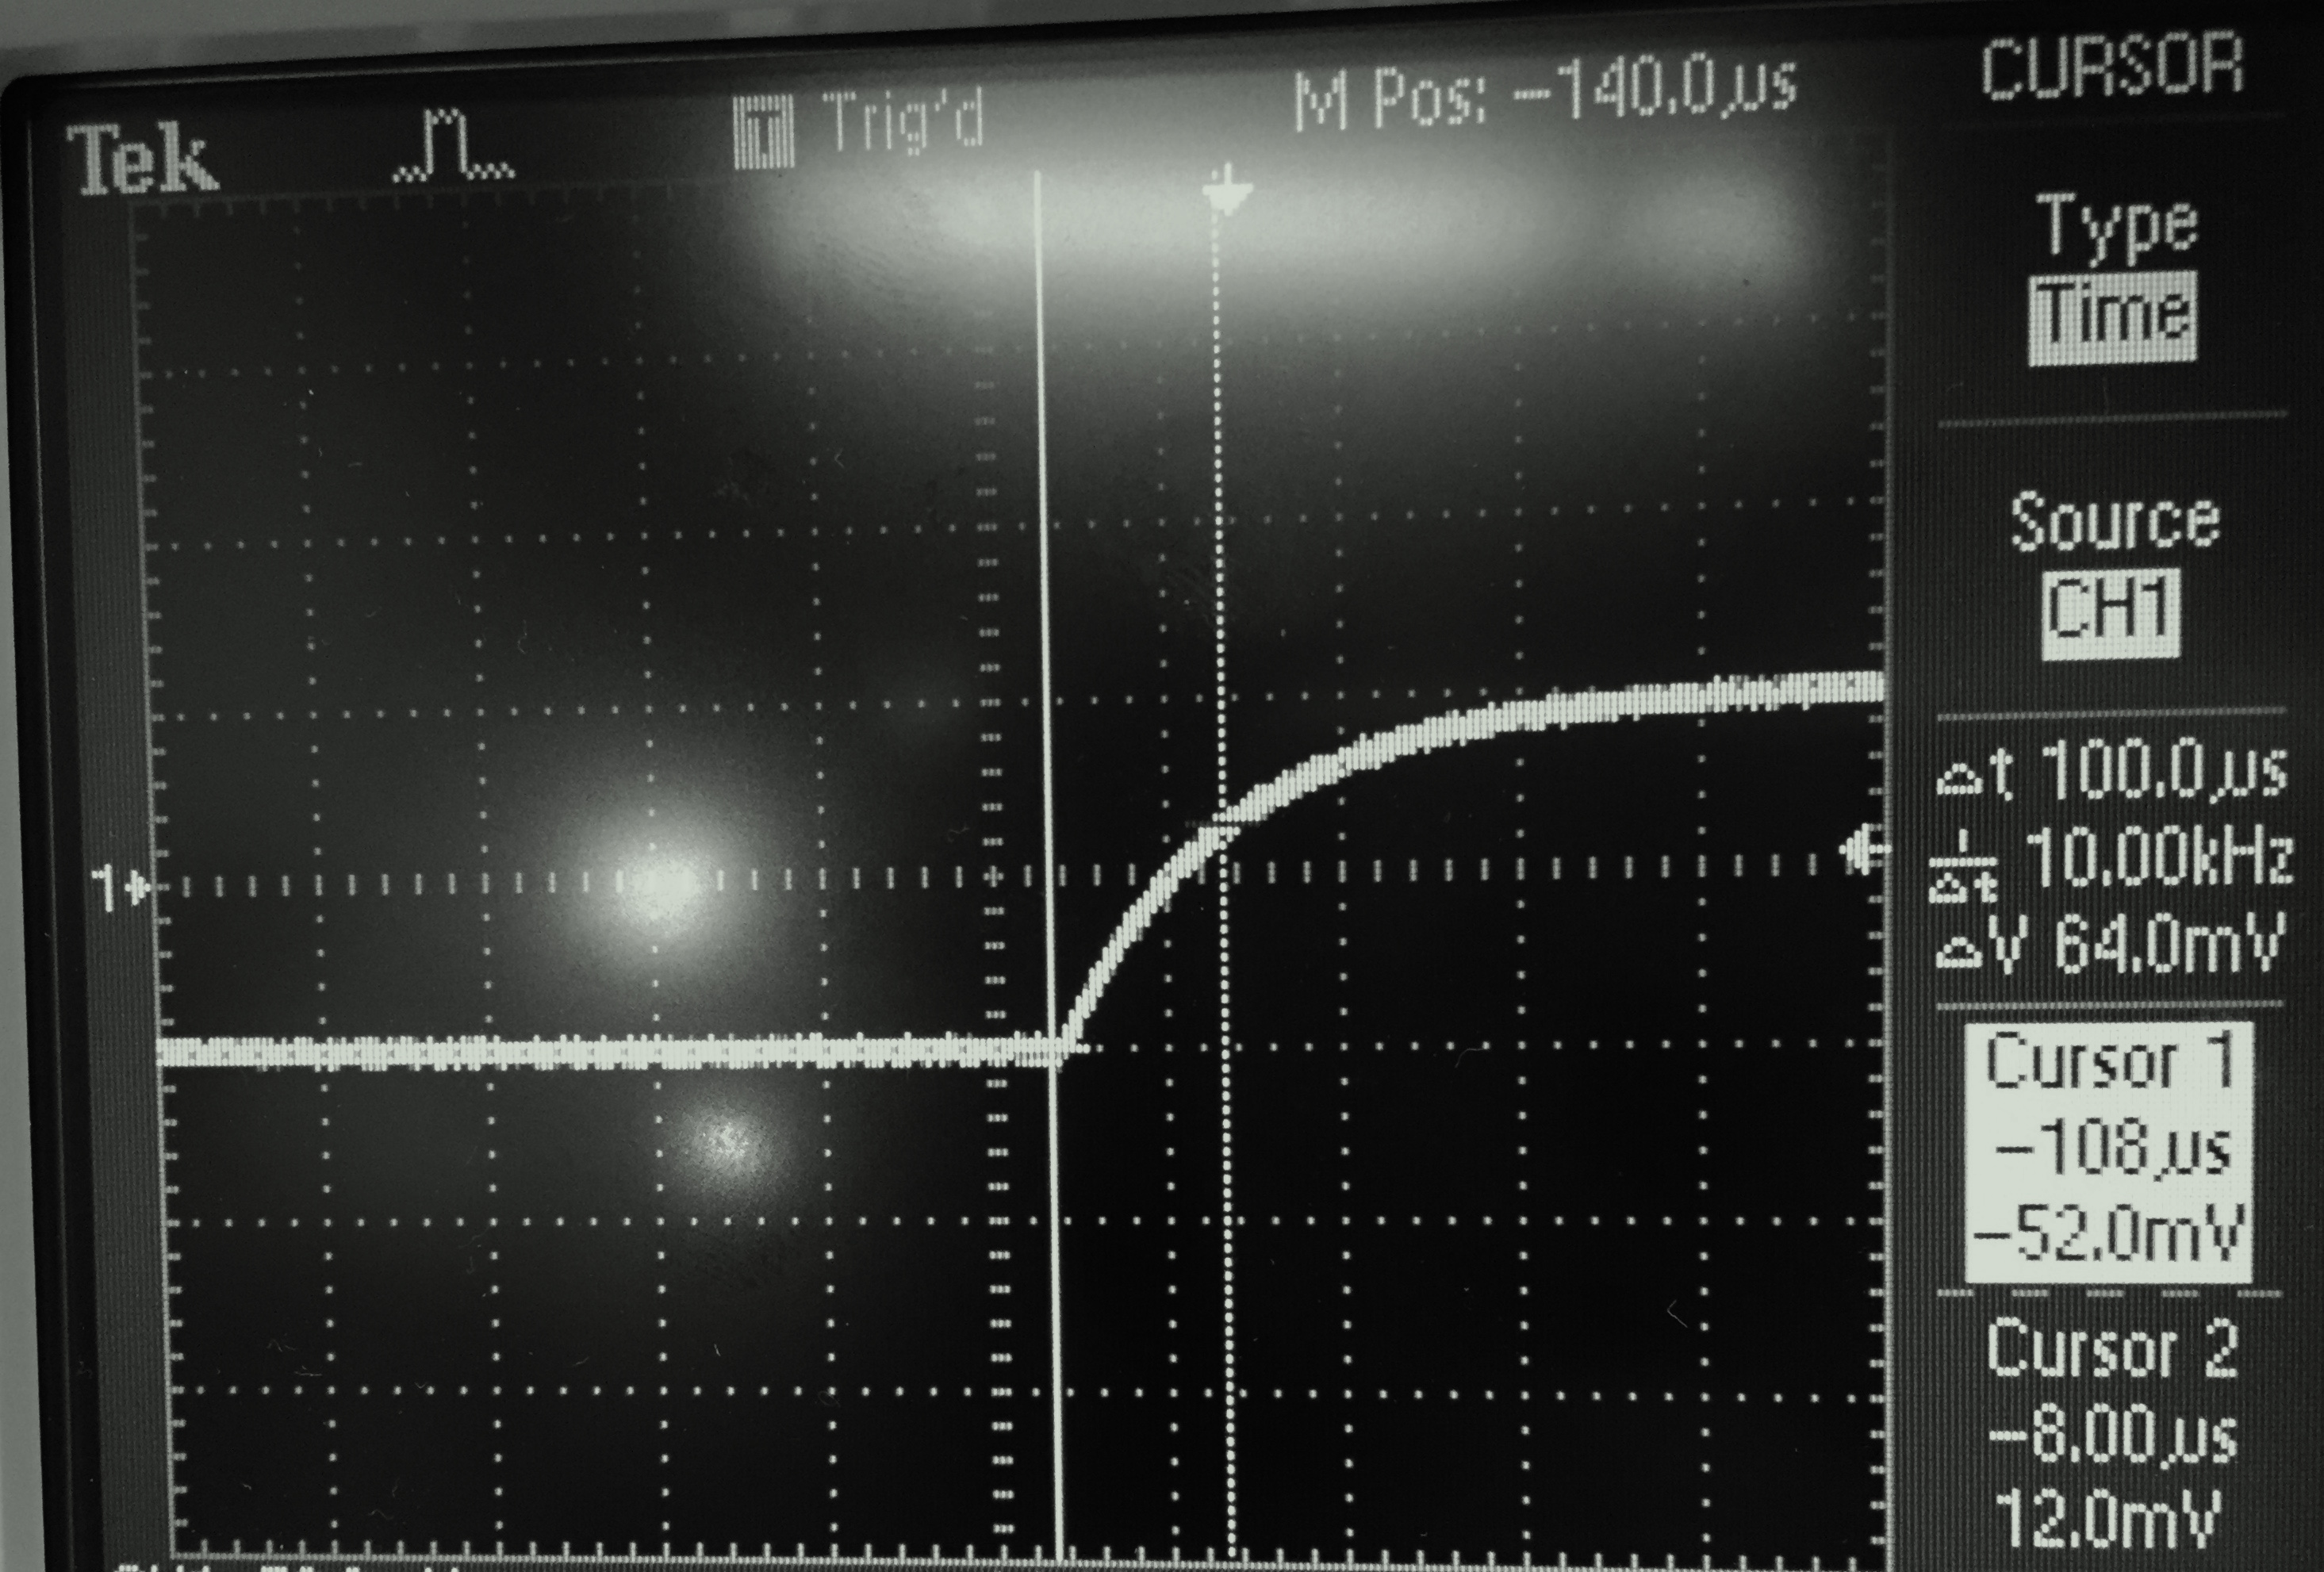
\includegraphics[scale=0.08]{lab2_risetime}\\
	 		Figure 1: Measuring rise time of the RC circuit
	 	\end{center}
	 	Similarly, to measure the fall time - the time required to go from 100\% to 37\% of the max voltage, we found the voltage that's at 37\% of the maximum and its time coordinate. The cursors gave us $\Delta t=108 \mu s$. So the rise time and fall time of the circuit are the same, both of which are close to the $100\mu s $ calculted RC time constant. The risetime and falltime are the same becayse the rate of charging up or discharging the capacitor should be identical. \\
	 	To explore the circuit in frequency domain, we varied the frequency by using the sweep function of the function generator to go from 10Hz to 20kHz. So we have a frequency f that varies with time t, and voltage that also varies with time. 
	
We built the RC differentiator circuit with a 100pF capacitor and 100$\Omega$ resistor, connecting the scope across the resistor to get the output signal. The function generator was also conencted to the scope so we could see the original input signal as well. 
\begin{center}
	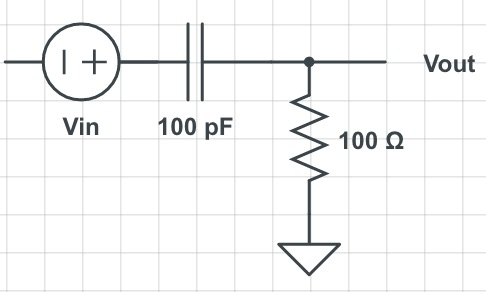
\includegraphics[scale=0.4]{lab2_differentiator}\\
	Figure 2: Differentiator RC circuit
\end{center}
	We drove the circuit with sine waves and sqaure waves (saw-tooth and square waves were hard to see on the scope). The scope displayed both the original input waves and the output waves to allow for comparison. 
	\begin{center}
		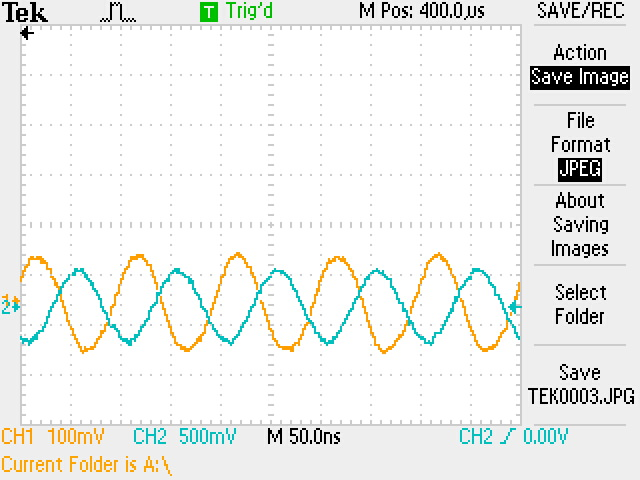
\includegraphics[scale=1]{lab2_c_sine}\\
		Figure 3: Sine waves inputted to Differentiator circuit
	\end{center}
	In Fig. 3 we can see that the two waves are nearly 90 degrees out of phase with each other, comfirming that the output signal was the derivative of sine wave, which is cosine wave.
		\begin{center}
			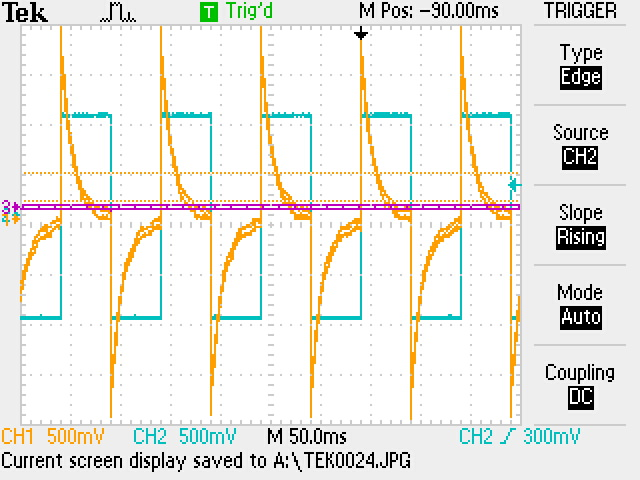
\includegraphics[scale=0.9]{f_square}\\
			Figure 4: Square waves inputted to Differentiator circuit
		\end{center}
	In Fig. 4 we see the original square wave and its derivative. The sharp peak of the differentiaed wave corresponds to the the veritcal part of the square wave which has infinity derivative. The differentiated wave drops from high peak to zero, correponding to the the horizontal part of the sqaure wave which has zero deritvative.\\
	This cirucit is a high-pass filter, because when the capacitor is charged up, no low-frequency DC voltage can pass through. So according to $z=\frac{1}{\omega RC}$, when the circuit is at 0 Hz, the input impedence is infinity. When it's at infinity frequency, the input impedence is zero. 
	\paragraph{ (d)}
	Similar to part (c), we built the integrator circuit with a 10k resistor and 0.01$\mu F$ capacitor, connecting the scope across the capcitor. 
\begin{center}
	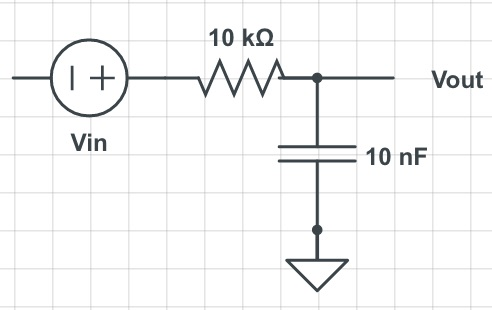
\includegraphics[scale=0.4]{lab2_integrator}\\
	Figure 5: Integrator RC circuit
\end{center}
We drove the circuit at 10kHz with sine, square, saw-tooth, and triangular waves. 
\begin{center}
	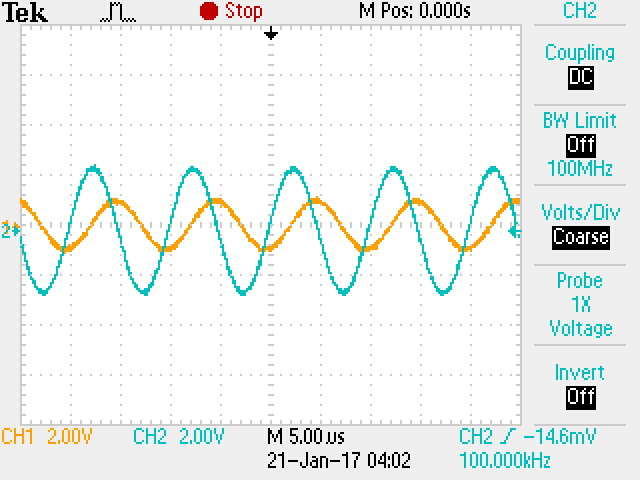
\includegraphics[scale=0.7]{d_sine}\\
	Figure 6: Sine wave inputted to integrator circuit
\end{center}
In Fig. 6 above, the higher amplitude is the orignal input sine wave, the other one is 90 degrees out of phase, meaning that it's the integrated cosine wave. \\ 
The expected amplitude of the sine wave is $A=\frac{1}{\sqrt(1+\omega^{2}R^{2}C^{2})}$, where we know the input frequency is f=10kHz, R=10k$\Omega$, C=0.01$\mu $F, and $\Omega=2\pi f$. So the calculated d amplitude is A=170mA. The measured amplitude is 192mA.
\begin{center}
	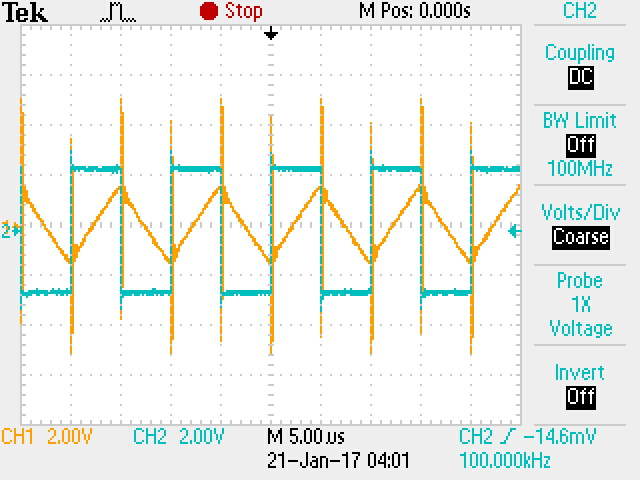
\includegraphics[scale=0.7]{d_square}\\
	Figure 7: Square wave inputted to Integrator circuit
\end{center}
In Fig. 7 above, we see the orginal square wave. The area under the square wave increases as we go across the positive part of the square, reaching a maximum. This corresponds to part of the integrated triangular wave that starts out at zero, increaes linearly, reaches a max. Similarly the area of the negative part of the square decreases from zero to a minimum.  This also corresponds to how the integrated triangular wave steadily decreases from the max to a nagative min. \\
\begin{center}
	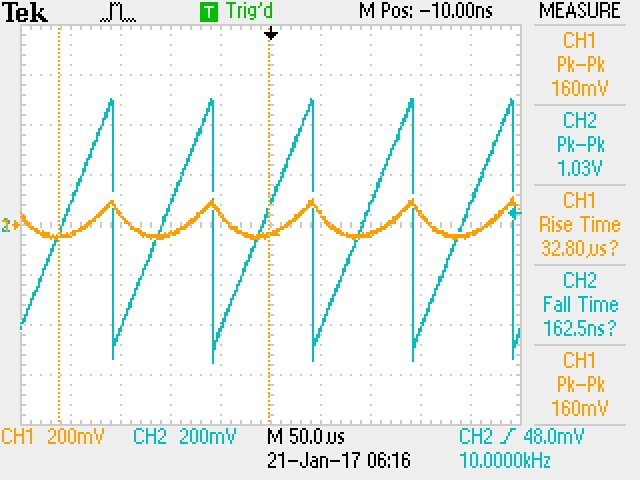
\includegraphics[scale=0.7]{d_sawtooth}\\
	Figure 8: Saw-tooth wave inputted to integrator circuit
\end{center}
In Fig.8, the original saw-tooth wave is shown along with the integrated wave. The integral of the slanted part of the saw-tooth shoud give a parabola kind-of curve with a sharp peak that correponds to the vertical part of the saw-tooth. And that's exactly the shape we have on the scope
\begin{center}
	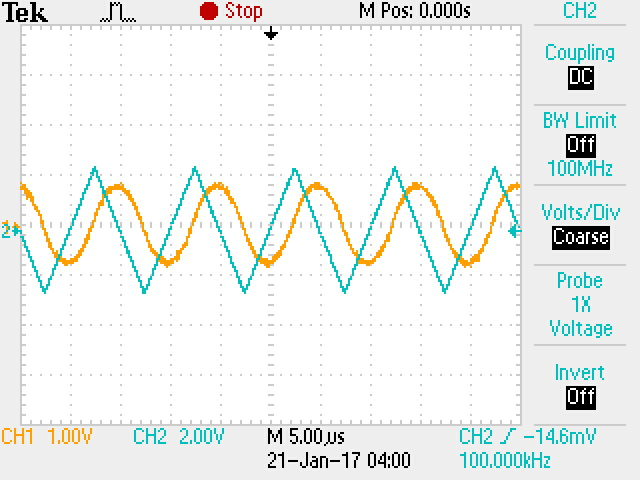
\includegraphics[scale=0.7]{d_triangular}\\
	Figure 9: Triangular wave inputted to Integrator circuit
\end{center}
Fig. 9  shows the orignal triangular wave. The integral of the triangular wave is similar to  the slanted part of the saw-tooth wave above, but the curve here should by vertically symmetrical to correspond to the symmetric triangular wave. So, the integrated curve, although it looks like a sine wave, is no the sine wave but 2nd degree polynomial curve.\\

	\paragraph{ (e)}
	We swept the circuit with sine waves from 1kHz to 3kHz in $\Delta t$=4s. So $\frac{\Delta f_{sweep}}{\Delta t_{sweep}}=\frac{2kHz}{4s}=\frac{1}{2}kHz/s$
	\begin{center}
		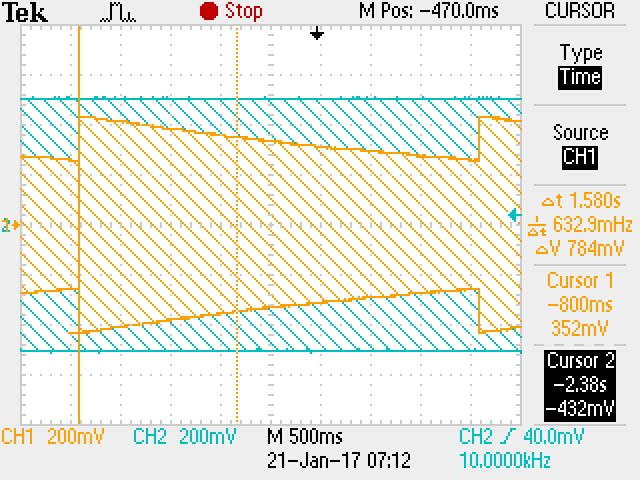
\includegraphics[scale=0.7]{e_sweep}\\
		Figure 10: Sweeping the low-pass filter to measure 3dB point
	\end{center}
	To find $f_{3dB}$, we need to first look for the maximum input voltage on the oscillascope, which is 500mV. So, $V_{3dB}=\frac{1}{\sqrt{2}} 500 mV=353.5 mV$. On the scope, with the help of cursors, we found that the time needed to go from 500mV to 353.5mV was 1.48s. So we can find $\Delta f=\frac{1}{2}kHz \times$ 1.48s=740Hz. Therefore, the measured $f_{3dB}=\Delta f+f_{start}= 740 Hz+1000Hz=1740 Hz.$ The calculated 3dB frequency is $f=\frac{1}{2\pi RC}=1590Hz$, which is close around the measured 3dB frequency. \\
	
	To look at the phase of the input and output waves in stop band, we drove the circuit (a low-pass filter) with a high frequency above the 3dB frequency. We obtained the signals in Fig.11, which shows the input and output waves 90 degrees out of phase, meaning that the high-frequency ouput signal has been integrated.
		\begin{center}
			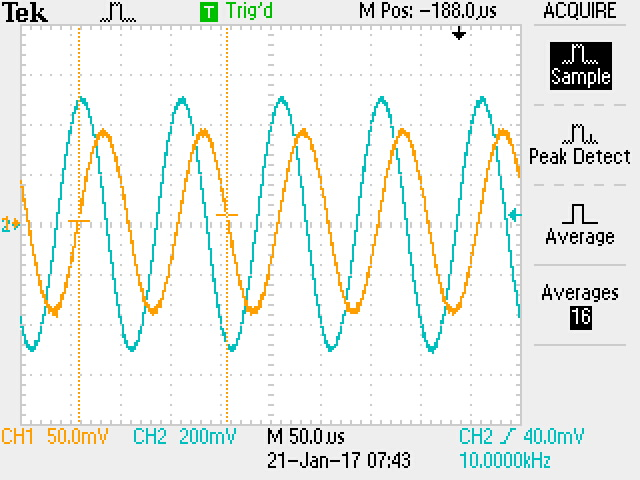
\includegraphics[scale=0.7]{e_stopband}\\
			Figure 11: Stop band of low-pass filter
		\end{center}
	To look at the pass band of the circuit, we drove it with a  low frequency. We would expect no phase difference because the low frequency wave should pass through this low-pass filter withou being integrated. Fig.12 below shows the signals we obtained,which match our expectation.
		\begin{center}
			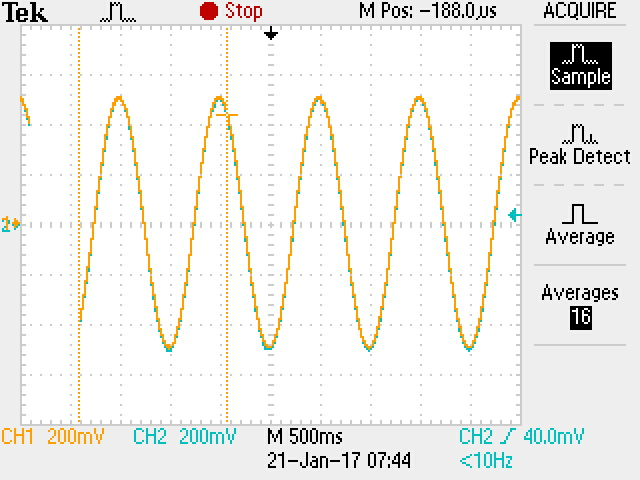
\includegraphics[scale=0.7]{e_passband}\\
			Figure 12: Pass band of low-pass filter
		\end{center}
	At a little above 3dB point, we can see that the signals in Fig. 13 are also exactly 90 degrees out of phase.
		\begin{center}
			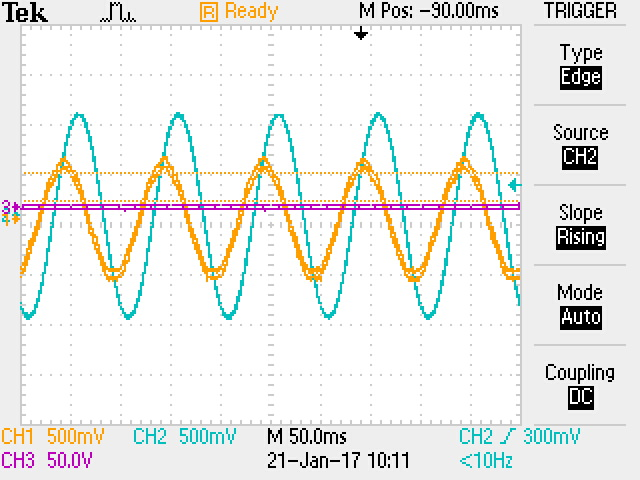
\includegraphics[scale=0.7]{e_3db}\\
		Figure 13: 3dB frequency of low-pass filter
	\end{center}
	6dB octave: On dB scale, going from 3dB to 6dB is doubling. Since $2 \times log(\frac{1}{\sqrt{2}}) = log(\frac{1}{2})$, so when the doubling on dB scale, the voltage should drop by 1/2. To confirm this, we first set the drive frequency at $f_{1}$=10kHz and recorded the voltage of the output signal $V_{1}$=32mV. Then we doubled the drive frequency to $f_{2}$=20kHz and recorded $V_{2}$=16mV. So, we see that when we doubled the frequency, the voltage indeed dropped by 1/2.\\
	
	Now we used the 3rd channel of the scope to look at SYNC output of the function generator. When we first set the trigger on the input sine wave, the scope only triggered at a specific voltage when the signal reached that trigger level. \\

	When we set the trigger on the SYNC signal, the scope will trigger constantly no matter what the trigger level we set it to be, just like when it's on auto trigger. It's better to trigger on SYNC instead of actual signal because this allows us to see the whole span of the signal wave on the horizontal axis. 
	\begin{center}
		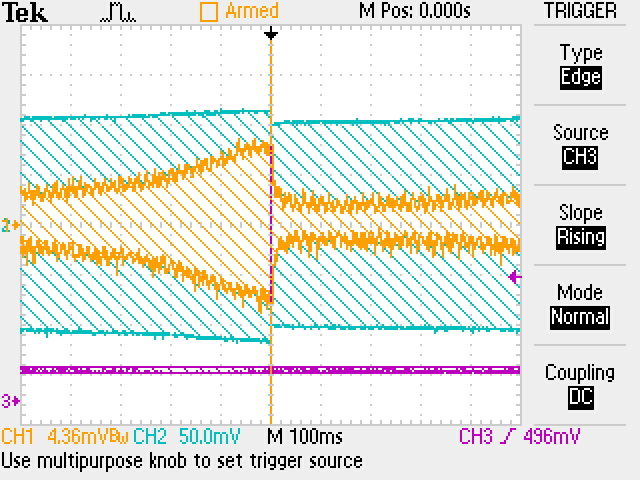
\includegraphics[scale=0.7]{e_sync}\\
		Figure 14: Triggering on SYNC pulse
	\end{center}
		
	\paragraph{ (f)}
	Switching the position of resistor and capacitor from the last part, we built a CR high-pass filter, which is also a differentiator. 
		\begin{center}
			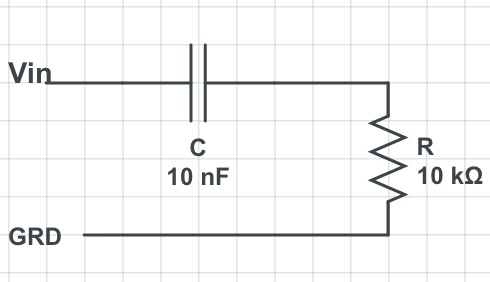
\includegraphics[scale=0.4]{f_circuit}\\
			Figure 15: CR high-pass filter circuit
		\end{center}
The 3dB point of this circuit is $f_{3dB}=\frac{1}{2\pi RC} \approx 200Hz$. To show that the cirucit works like a high pass filter, we first passed a low frequency below 200 Hz. We saw the input square wave being differentiated. The derivative of the square wave at the edge of the sqaure is either zero or infinity, which is what we saw on the scope (Fig. 16).
	\begin{center}
		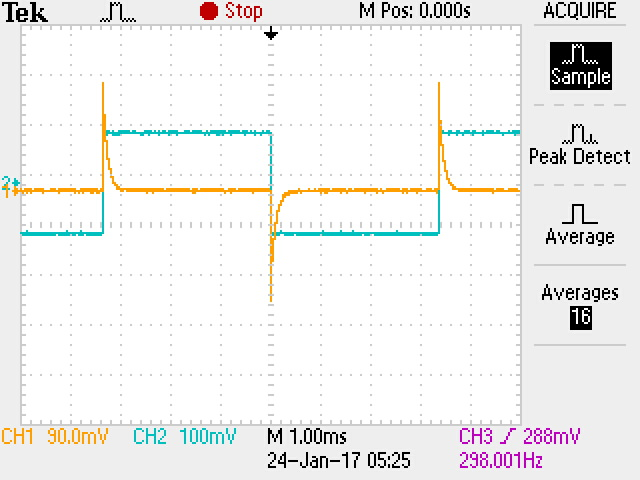
\includegraphics[scale=0.7]{f_hipass}\\
		Figure 16: Low-frequency square wave inputted to high-pass filter
	\end{center}
When we passed a high-frequency wave at above 90k Hz, the signal should pass through without being differentiated. So the input and output signals should look the same, which is what we saw on the scope (Fig.17).
	\begin{center}
		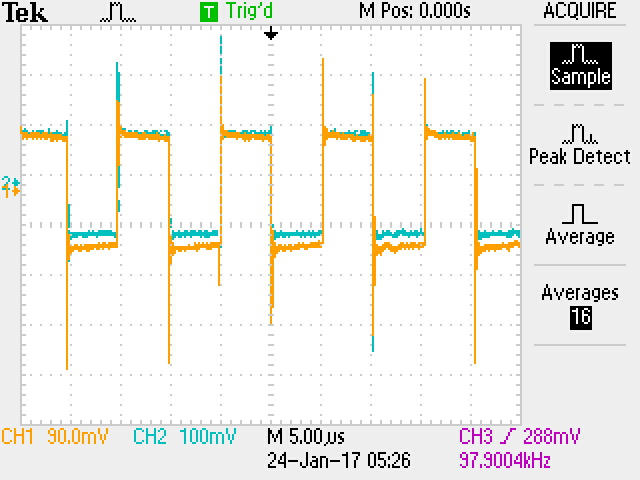
\includegraphics[scale=0.7]{f_hipass2}\\
		Figure 17: High-frequency square wave inputted to high-pass filter
	\end{center}
	Next, we put the SYNC output to the scope and set the trigger on it. We set the sweep from 10Hz to 200k Hz, and time to 1s. Now we could easily get the 3dB point from the scope (Fig. 18) by using the cursors to find the time at $V_{max}$ and time at $V_{3dB}$.
		\begin{center}
			\includegraphics[scale=0.8]{f_3db}\\
			Figure 18: Triggering off SYNC to find 3dB point
		\end{center}
		 
	\paragraph{ (g)}
We put a 1 kHz signal through the leads on one side of the transformer and measured output the signal from the other outer leads. The input voltage and output voltage were the same, but inverted (Fig. 19). So the voltage ratio of this transformer is 1:1. We tested over a large frequency range on the function generator and found the range over which the transformer works as expected is 10Hz to 9.99 kHz. \\ 
Then we put the signal back to 1 kHz, and found the output signal between the outer lead and center-tap was 2:1. This is because when we connected to the center-tap, only half of the coils is used. Since the number of coil turned is directly proportional to the votlage induced, the output voltage should be half of the orginal input.
	\begin{center}
		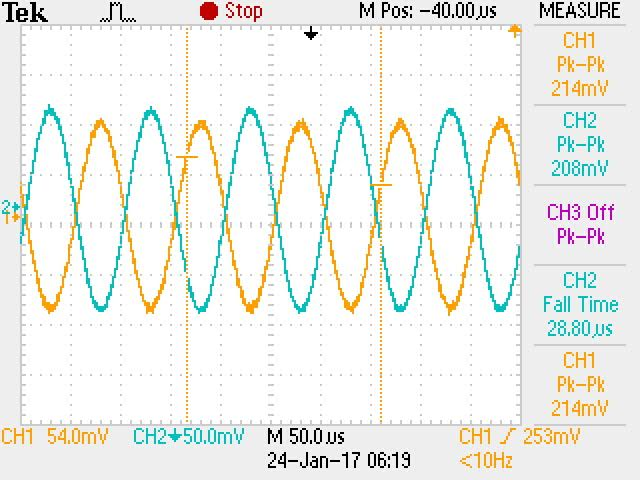
\includegraphics[scale=0.3]{g_1to1}\\
		Figure 19: Input and output of a 1 to 1 transformer.
	\end{center}

	\paragraph{ (h)}
	We connected a 10:1 transformer to the AC power supply on the wall and built the following circuit. 
		\begin{center}
			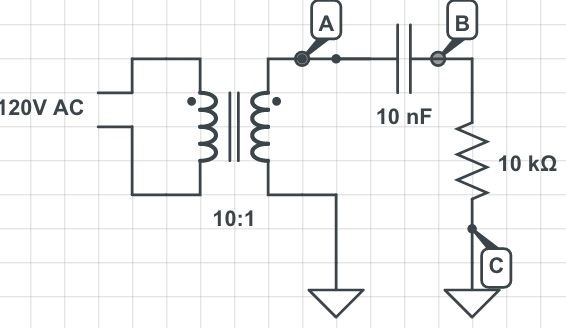
\includegraphics[scale=0.4]{h_transf}\\
			Figure 20: Input and output of 1 to 1 transformer.
		\end{center}
The frequency output at A was 60.02 Hz according to the scope. The input voltage at A was $V_{in}=33.0V$, the output voltage at B was $V_{out}=2.12V$. The peak to peak votlage input was 33.0V,  so the voltage of just 1 peak is $\frac{33}{2}V$. The RMS voltage is, therefore, $V_{rms}=\frac{33}{2}V \times (\frac{1}{\sqrt{2}})=11.7V$, which is close to the 11V RMS voltage on the back of the power supply. The attenuation at 60 Hz is $10log(\frac{V_{out}}{V_{in}})=10log(\frac{2.12V}{33.0V})=-23.84 dB$. 
	
	\paragraph{ (i)}
Electrolytic capacitors have polarity because of the way they are made. The dielectric material used in the capacitors are made by polarization, and we use this dielectric film becuase allows for much larger capacitance in the same volume. \\
We contructed a high-pass filter (Fig. 21) with a 4.7$\mu F$ electrolytic capacitor and resistors. This circuit is also a voltage divider (the part in the red box in Fig.21). 
	\begin{center}
		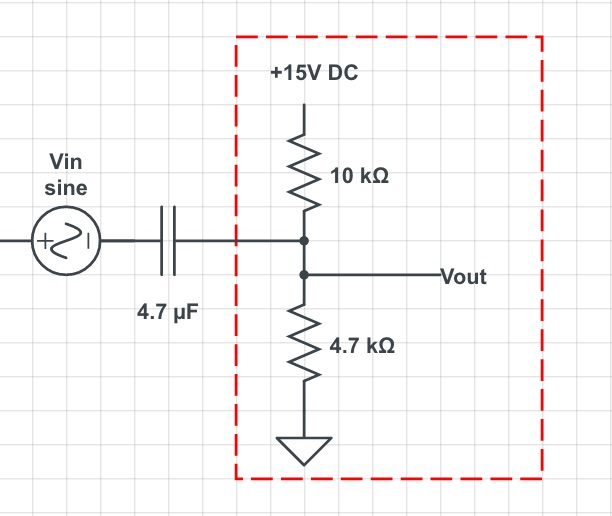
\includegraphics[scale=0.3]{i_circuitA}\\
		Figure 21: Circuit A: a high-pass filter and voltage divider 
	\end{center}
The input DC voltage is 15V, first resistor is 10k, and the second resistor is 4.7k. So the voltage drop at $V_{out}$ should be around 5V. Now we also have 1V 20kHz AC voltage from the function generator. So the total votlage at $V_{out}$ should be swinging around 5V(from DC)$\pm$ 1V (from AC)=4-6V. We measured the output signal on the scope along with the original input signal (Fig.22). 
		\begin{center}
			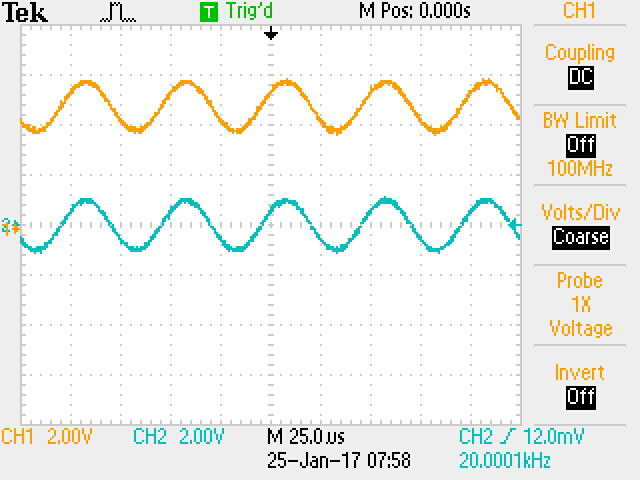
\includegraphics[scale=0.7]{i_top}\\
			Figure 22: Input and output ignals of cirucit A
		\end{center}
In Fig.22 we can clearly see the input voltage oscillating between $\pm 1V$ while the output signal oscillate around 4-6V as expected. \\
We then built the blocking circuit B with a electrolytic 4.7$\mu F$ capacitor and a 100k resistor, which make a high-pass filter. Then we added circuit B to circuit A. 
	\begin{center}
		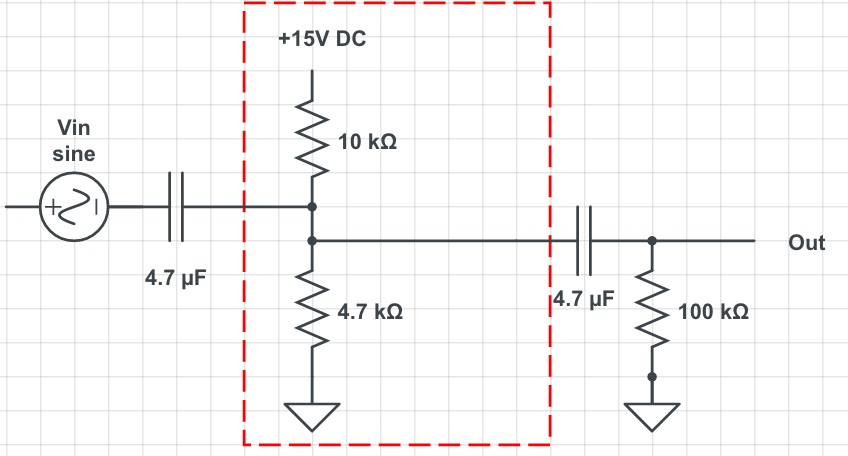
\includegraphics[scale=0.26]{i_circuitAB}\\
		Figure 23: Blocking circuit B added to circuit A.
	\end{center}
Blocking circuit B should filter out the low frequency 5V signal from the DC source, so only the 1V AC voltage from function generator should remain. When we measured the output signal, we saw indeed the output signal only oscillate around $\pm$1V (Fig.24).
\begin{center}
	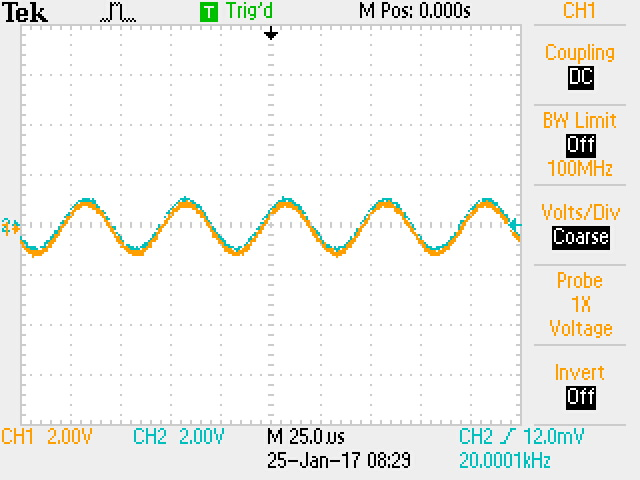
\includegraphics[scale=0.7]{i_ABsignal}\\
	Figure 24: Input and output signals of circuit A and B
\end{center}
To find out the low frequency limit of this blocking circuit, we tested different frequencies on the function generator and found that, at or below 100Hz the signal started to die off. 
\begin{center}
	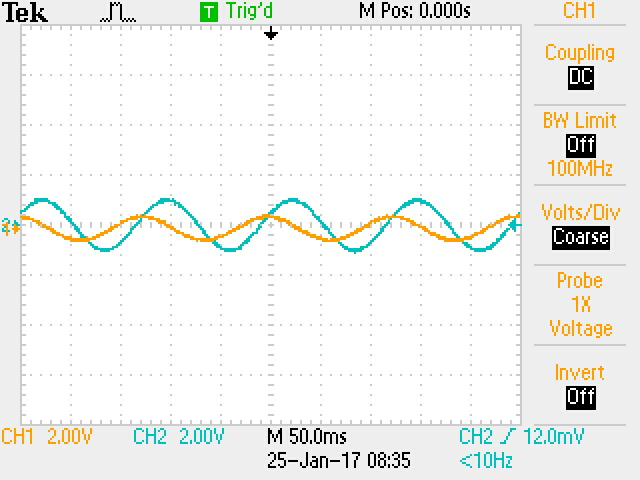
\includegraphics[scale=0.7]{i_lowfreq}\\
	Figure 25: Low frequency limit of the blocking circuit
\end{center}
Lasatly, we put circuit A on AC coupling, and we saw that it produce the same effect to the low frequency signal  as the circuit B did.
\begin{center}
	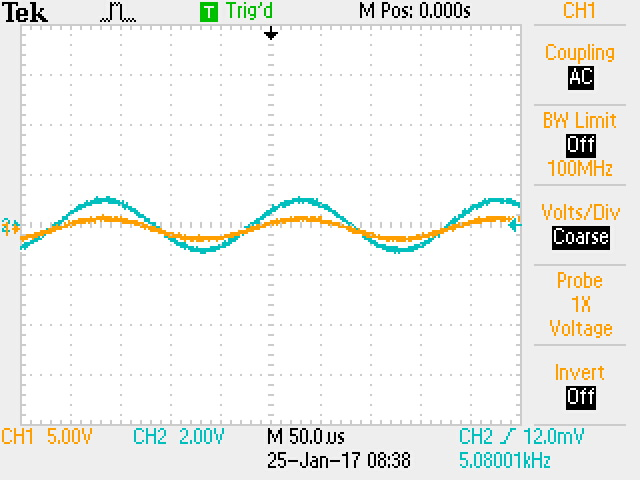
\includegraphics[scale=0.7]{i_ac}\\
	Figure 26: AC coupling on circuit A
	\end{center}
\end{document}
